\clearpage
\begin{landscape}
\setlength{\intextsep}{4bp}
\section{แผนภาพฐานข้อมูลระบบใบลา}\label{app:db}
\begin{figure}[H]
\centering
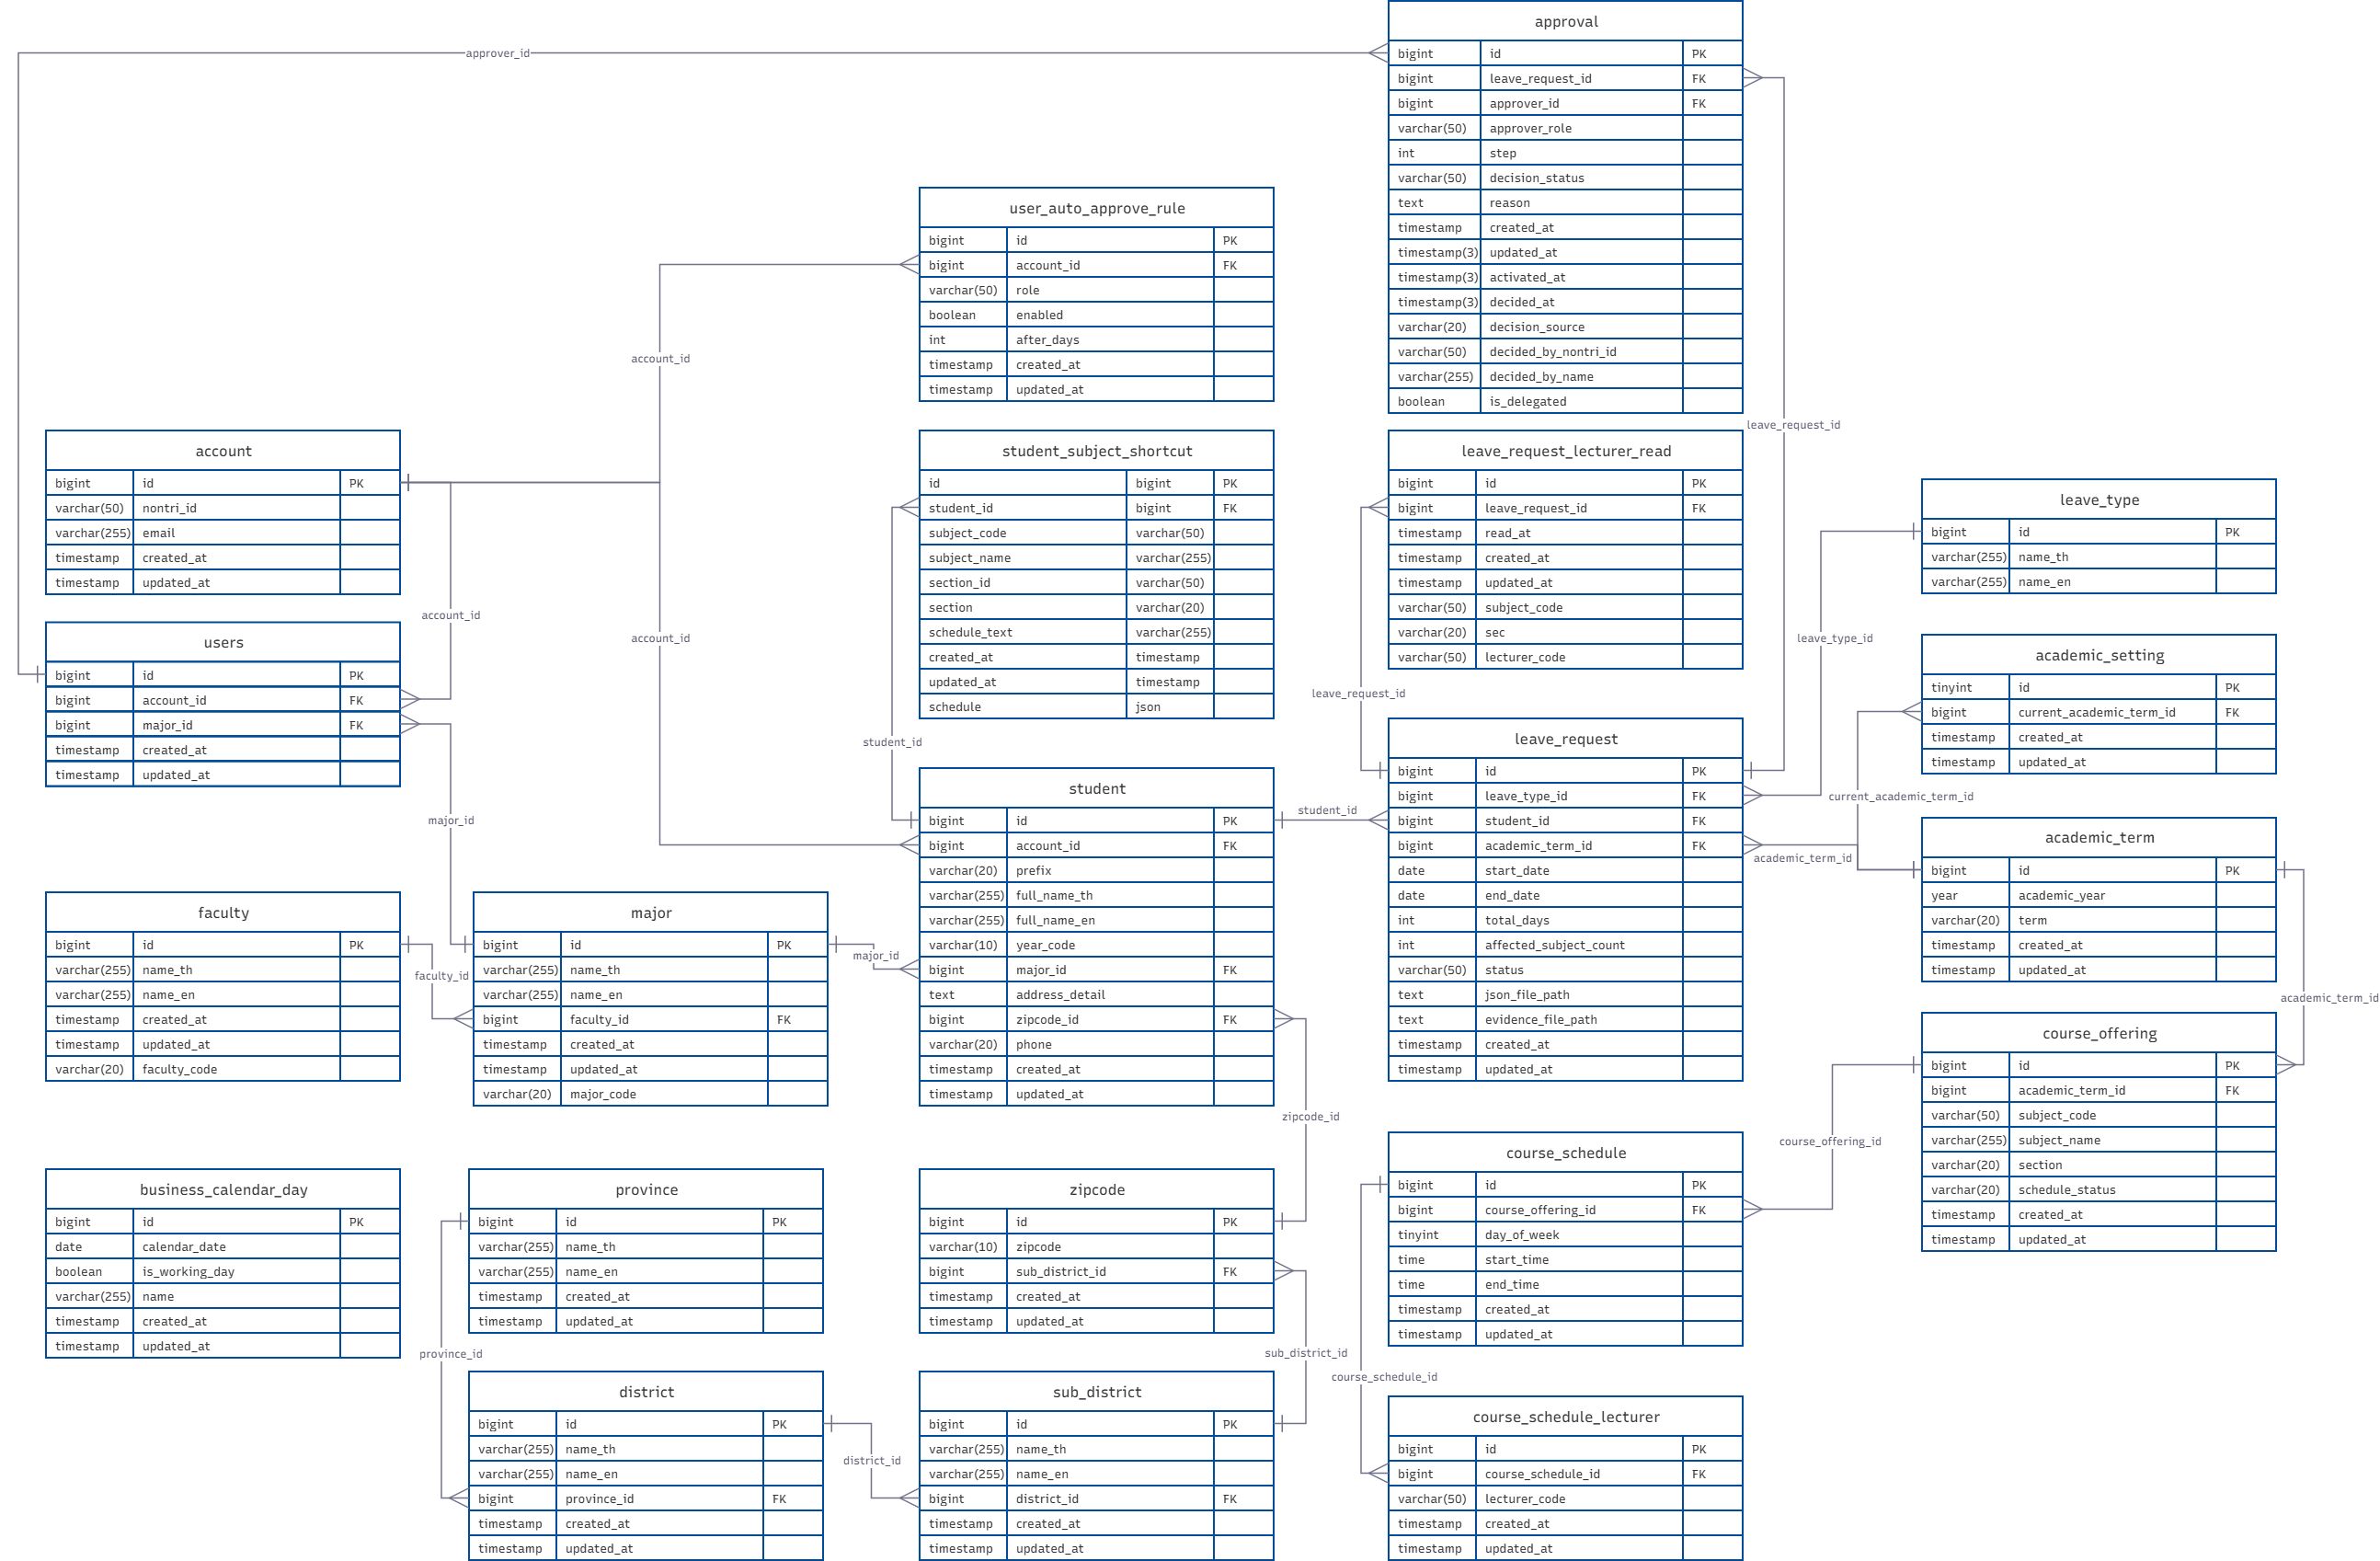
\includegraphics[width=\linewidth,height=148mm,keepaspectratio]{images/leave-schema/DB.png}
\caption{โครงสร้างฐานข้อมูลระบบใบลา}\label{fig:db-original}
\end{figure}
\clearpage
\section{ภาพรวมคลังข้อมูลรายงาน}\label{app:dw-overview}
\begin{figure}[H]
\centering
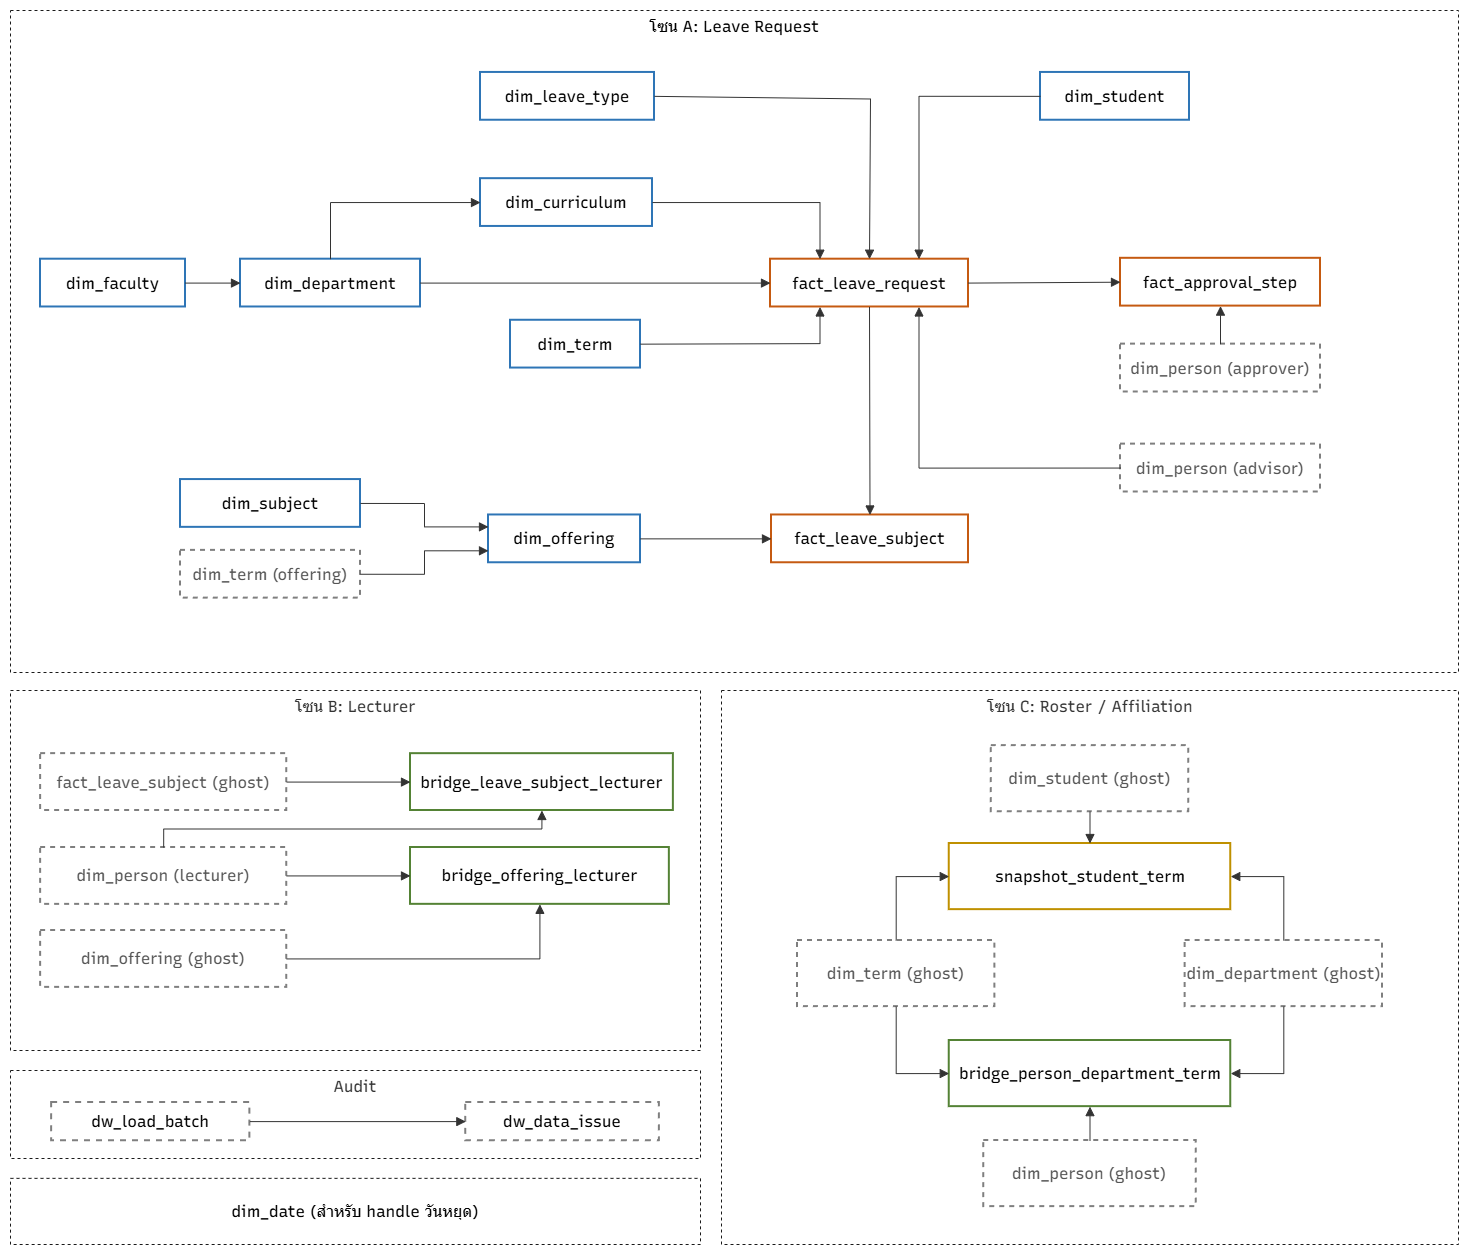
\includegraphics[width=\linewidth,height=148mm,keepaspectratio]{images/leave-schema/DW-OVERVIEW.png}
\caption{ภาพรวมองค์ประกอบคลังข้อมูลรายงาน}\label{fig:dw-overview-original}
\end{figure}
\clearpage
\section{แผนภาพความสัมพันธ์คลังข้อมูล}\label{app:dw-detail}
\begin{figure}[H]
\centering
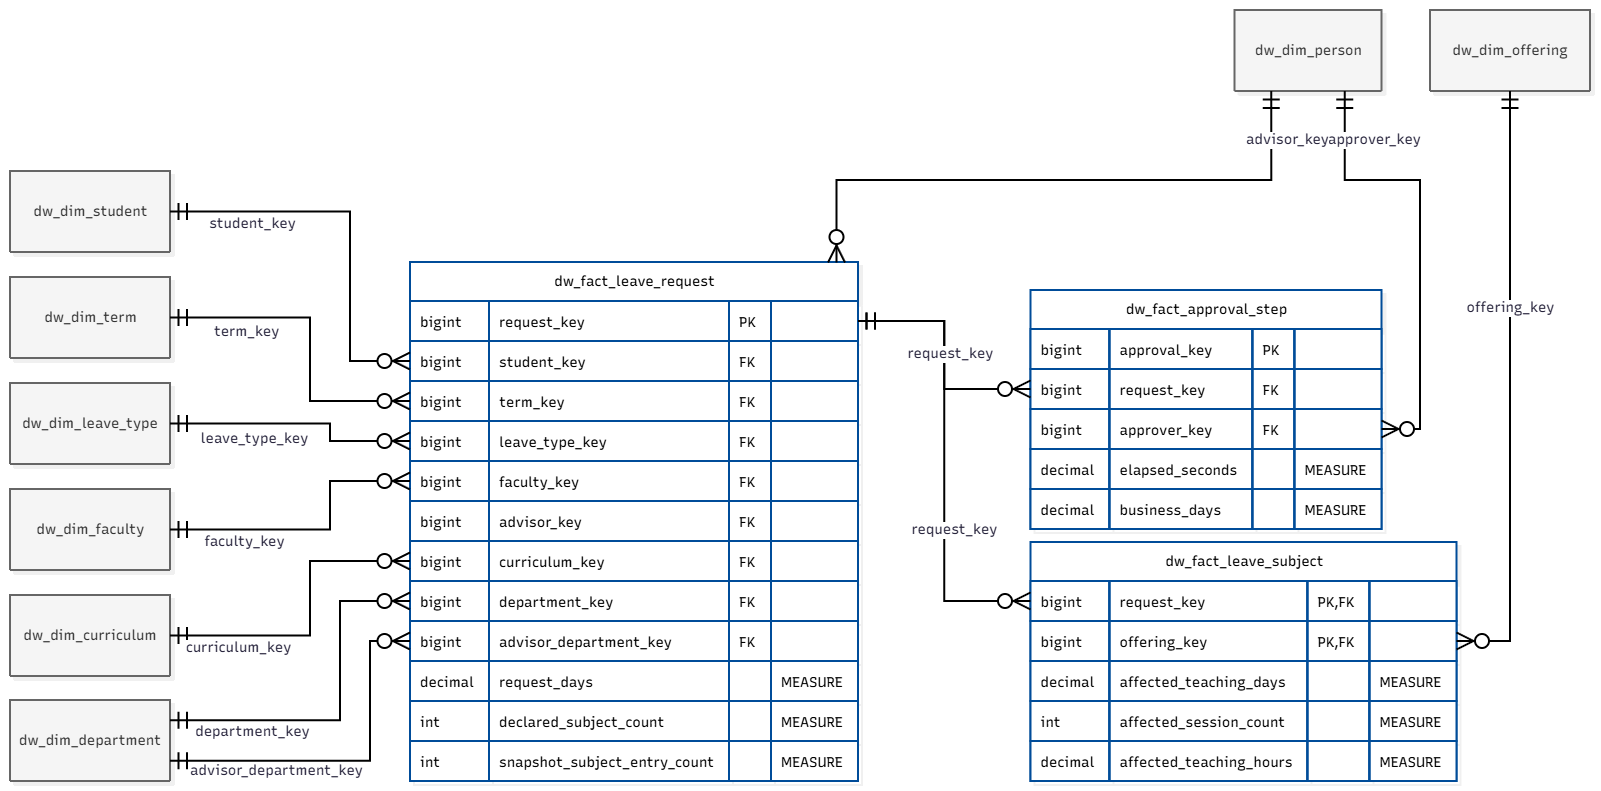
\includegraphics[width=\linewidth,height=148mm,keepaspectratio]{images/leave-schema/DW-ERD.png}
\caption{ความสัมพันธ์ของข้อมูลในคลังข้อมูลรายงาน}\label{fig:dw-erd-original}
\end{figure}
\clearpage
\section{แผนภาพคลังข้อมูลฉบับเต็ม}\label{app:dw-full}
\begin{figure}[H]
\centering
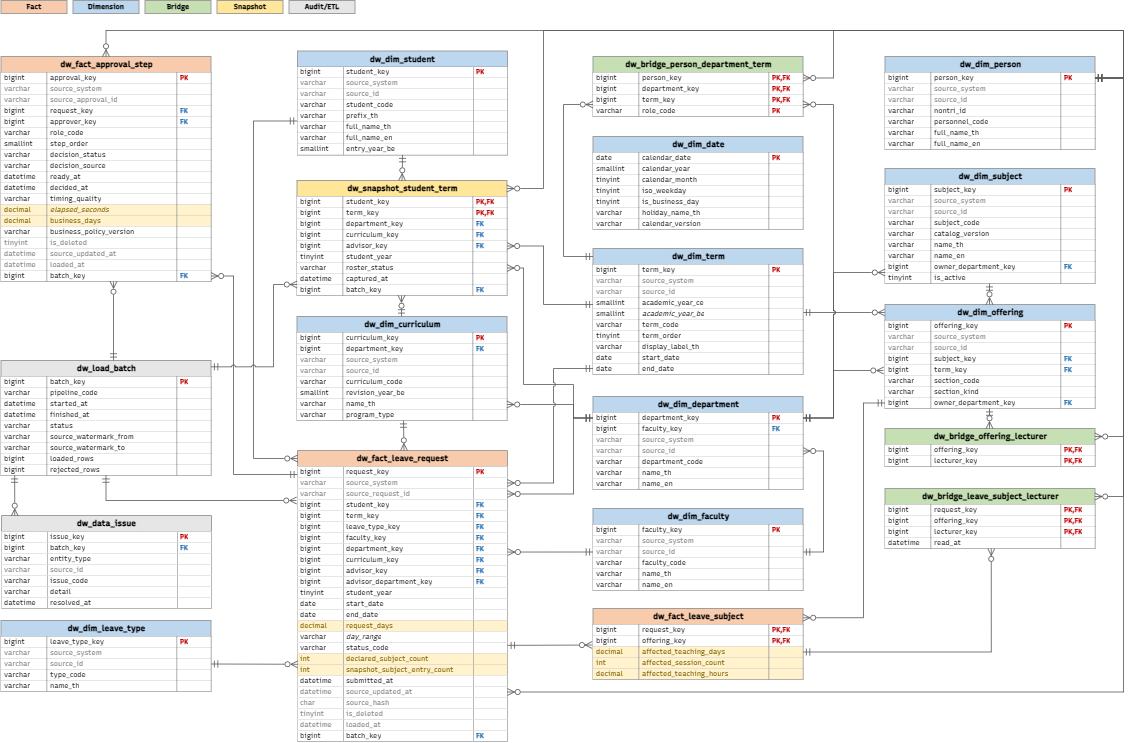
\includegraphics[width=\linewidth,height=148mm,keepaspectratio]{images/leave-schema/DW-FULL_VERSION_2.png}
\caption{โครงสร้างคลังข้อมูลรายงานฉบับเต็ม}\label{fig:dw-full-original}
\end{figure}
\clearpage
\section{แผนภาพส่วนควบคุมคลังข้อมูล}\label{app:controls}
\begin{figure}[H]
\centering
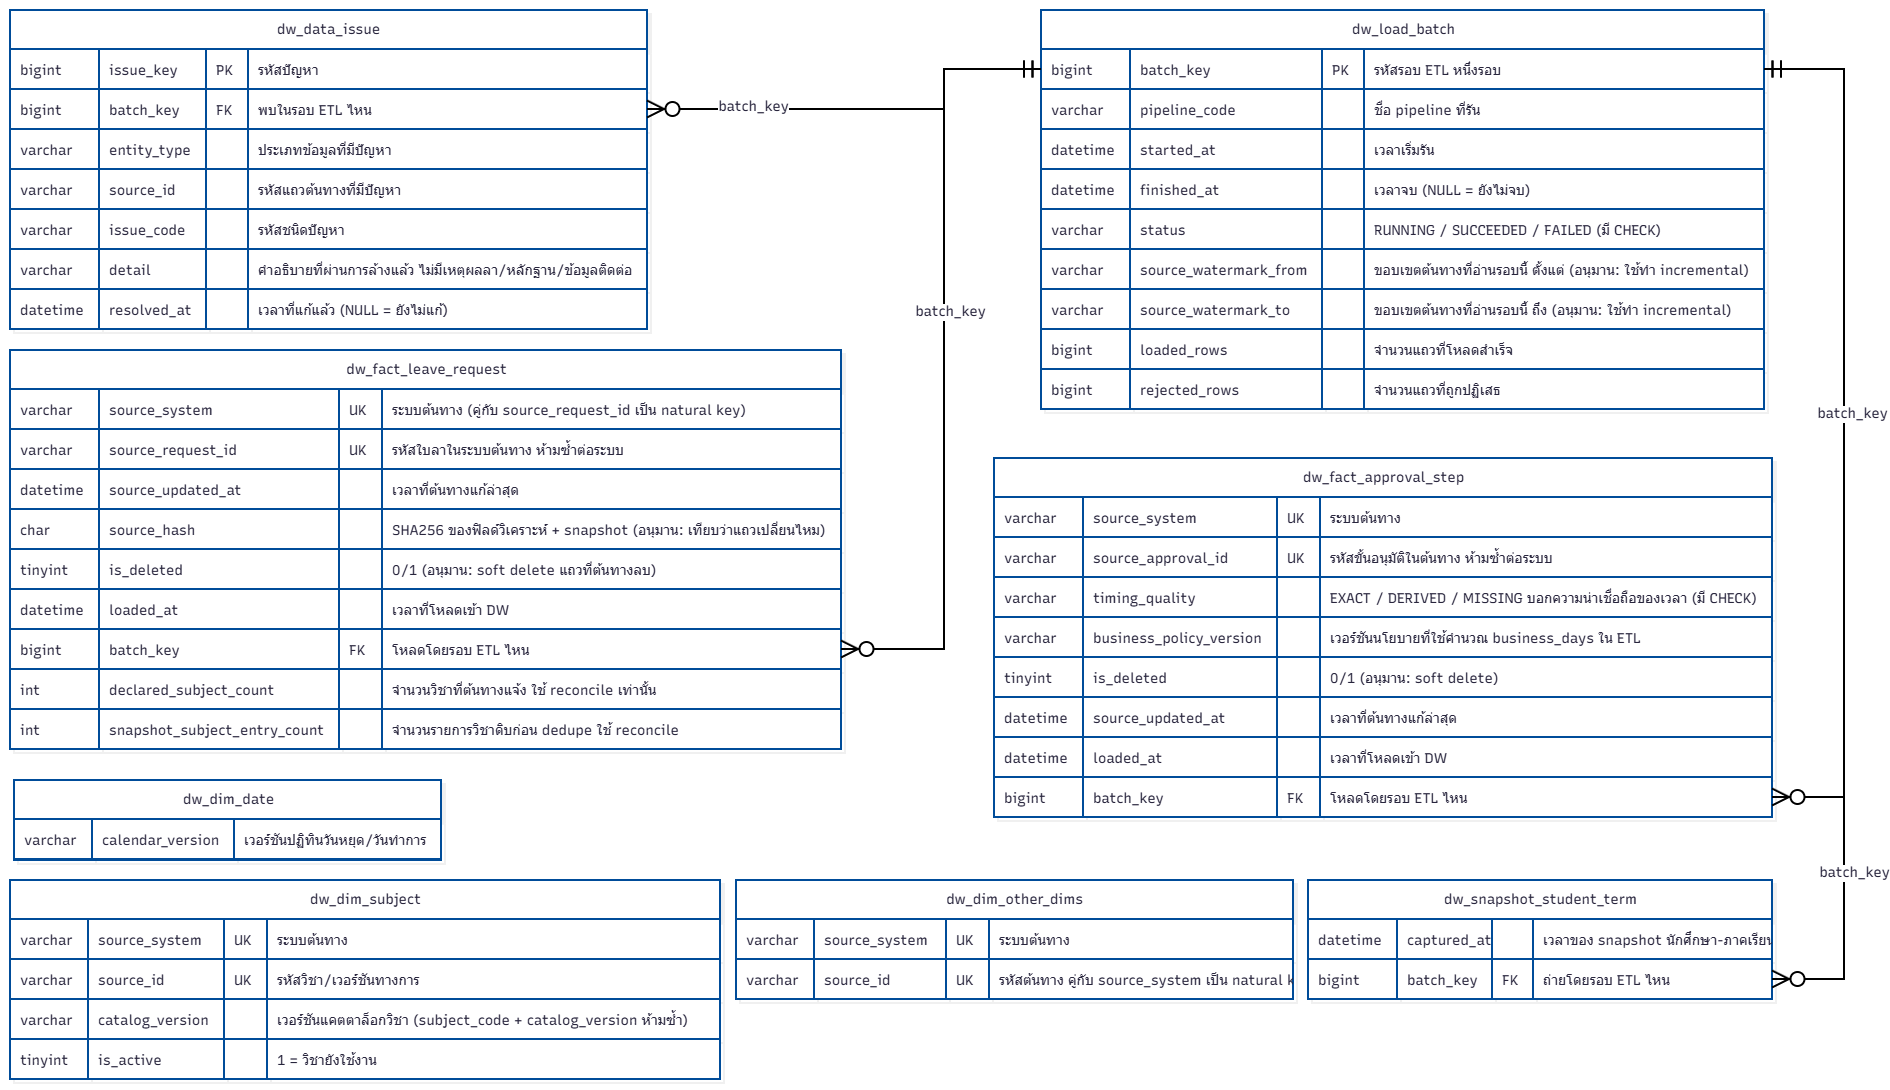
\includegraphics[width=\linewidth,height=148mm,keepaspectratio]{images/leave-schema/DW-CONTROL_COLUMNS.png}
\caption{ส่วนควบคุมการปรับปรุงข้อมูลในคลังข้อมูล}\label{fig:dw-control-original}
\end{figure}
\end{landscape}
